\documentclass{article}

% set font encoding for PDFLaTeX or XeLaTeX
\usepackage{graphicx}
\usepackage{ifxetex}
\usepackage{hyperref}

\ifxetex
  \usepackage{fontspec}
\else
  \usepackage[T1]{fontenc}
  \usepackage[utf8]{inputenc}
  \usepackage{lmodern}
\fi
\title{Actividad 2}
\author{Fisica Computacional 1\\
Corral Valdez Jesus Giovanni\\
Departamento de Física\\
Universidad de Sonora}
\date{}
% Enable SageTeX to run SageMath code right inside this LaTeX file.
% documentation: http://mirrors.ctan.org/macros/latex/contrib/sagetex/sagetexpackage.pdf
% \usepackage{sagetex}

\begin{document}
\maketitle
\clearpage
\section{Introducción}
La presente actividad fue un comienzo a lo que aprenderemos el resto del semestre, el "Análisis de datos". Por medio de Jupyter Notebook con lenguaje python se analizará los ultimos días de una base de datos y se realizara gráficas de estos datos.\\
Los datos fueron recolectados por Estaciones Meteorológicas Automáticas (EMAS, \url{http://smn.cna.gob.mx/es/emas}). Estos nos aportan datos sobre presión, altitud, temperatura y otras cosas importantes cada cierto tiempo sobre una estaciòn de México.\\
\section{Desarrollo}
1.Se descargó los registros de una estación metereológica, en este caso de Puerto Peñasco.\\
2.Por medio de Excel se cambio el formato a Csv.\\
3.En Jupyter Notebook se comenzó el código para analizar los datos, abriendo el csv, checando que la exportación haya sido la correcta.\\
\begin{figure}[h]
  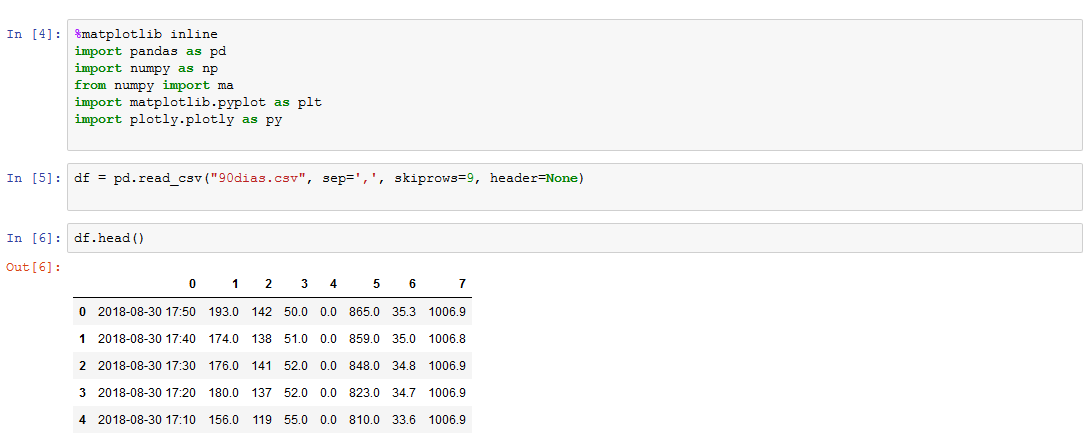
\includegraphics[width=\linewidth]{2-01.png}
\end{figure}
\\
4.Se le asignó un nombre a las columnas y nos fijamos en que tipo son cada uno.\\
\begin{figure}[h]
  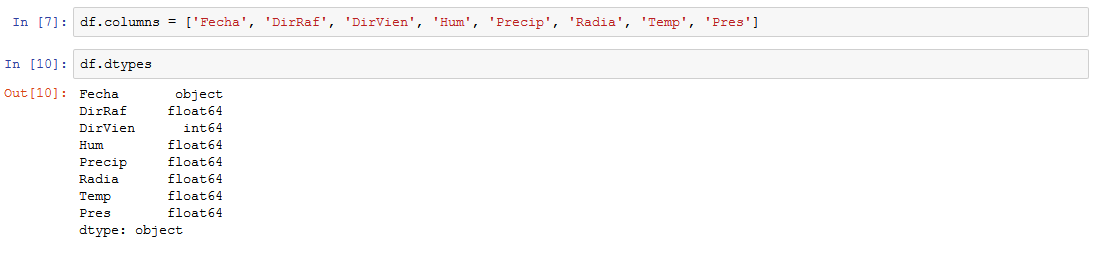
\includegraphics[width=\linewidth]{2-02.png}
\end{figure}
\\
\clearpage
5.Por conveniencia, preferimos tener la columna de fecha en formato de datetime asi que lo cambiamos.\\
\begin{figure}[h]
  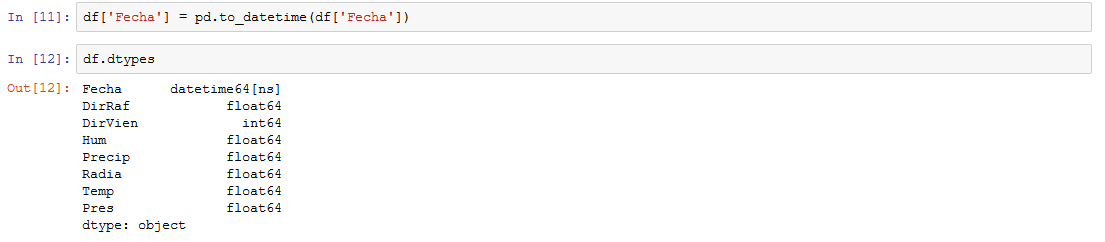
\includegraphics[width=\linewidth]{2-03.png}
\end{figure}
\\
6.Por como estan dados los datos por las estaciones, el numero mas arriba en la lista es el dato mas nuevo, pero si queremos graficar de preferencia esperamos que el primer dato sea la fecha mas vieja asi que tenemos que invertir la tabla (en la imagen anterior mostramos la cola de la tabla).\\
\begin{figure}[h]
  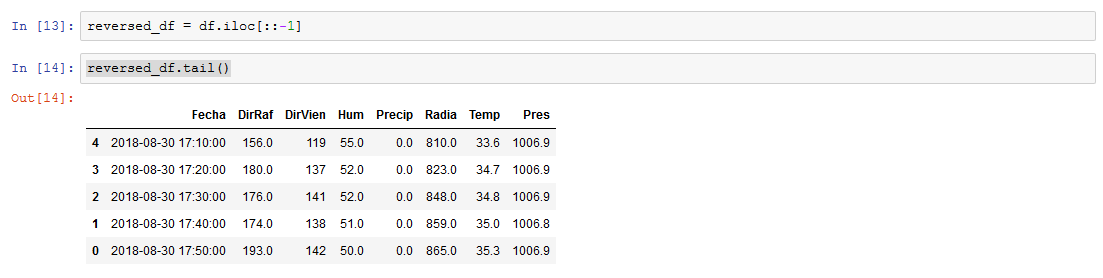
\includegraphics[width=\linewidth]{2-04.png}
\end{figure}
\\
7.Por estetica, reiniciamos los índices de los datos ya que al invertirlo, el ultimo dato tenia el numero 1.\\
\begin{figure}[h]
  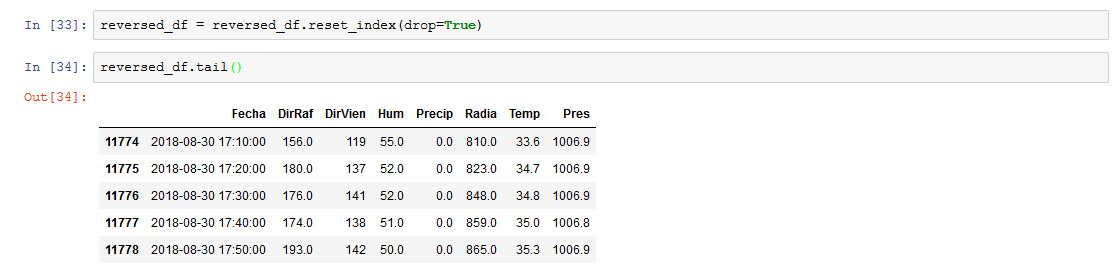
\includegraphics[width=\linewidth]{2-05.png}
\end{figure}
\\
\clearpage
8.Una gráfica de la temeperatura respecto al tiempo, pero al ser tantos dias lo que se esta graficando no se aprecía bien.\\
\begin{figure}[h]
  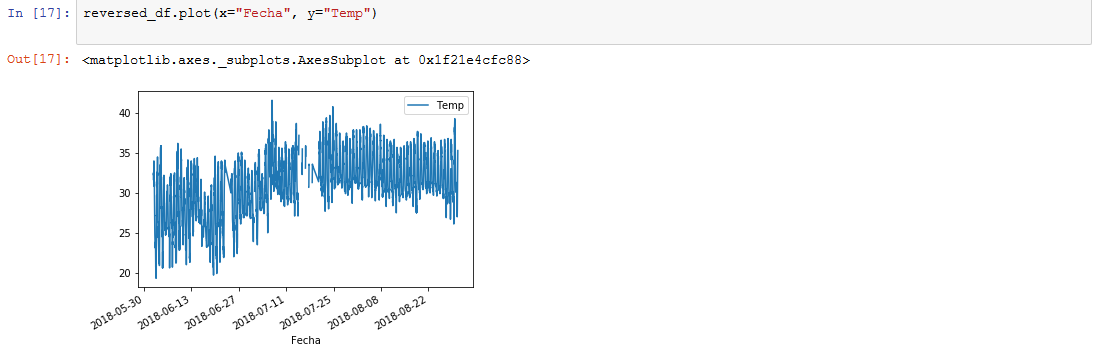
\includegraphics[width=\linewidth]{2-06.png}
\end{figure}
\\
9.Por lo tanto, lo que haremos es restringir el tiempo a solo 10 días.\\
\begin{figure}[h]
  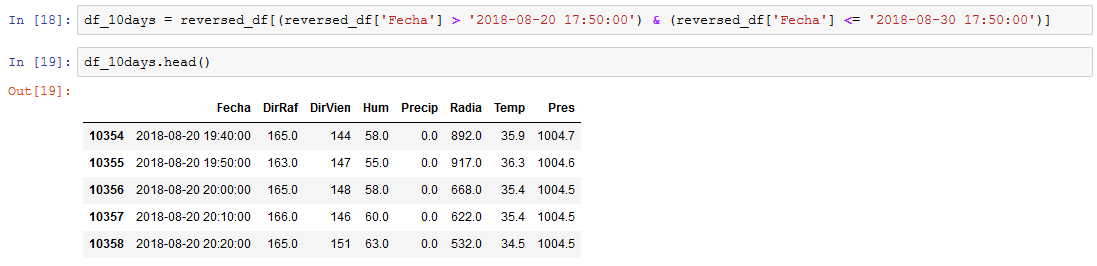
\includegraphics[width=\linewidth]{2-07.png}
\end{figure}
\\
10. Gráfica de la temperatura en el intervalo de 10 días.
\begin{figure}[h]
  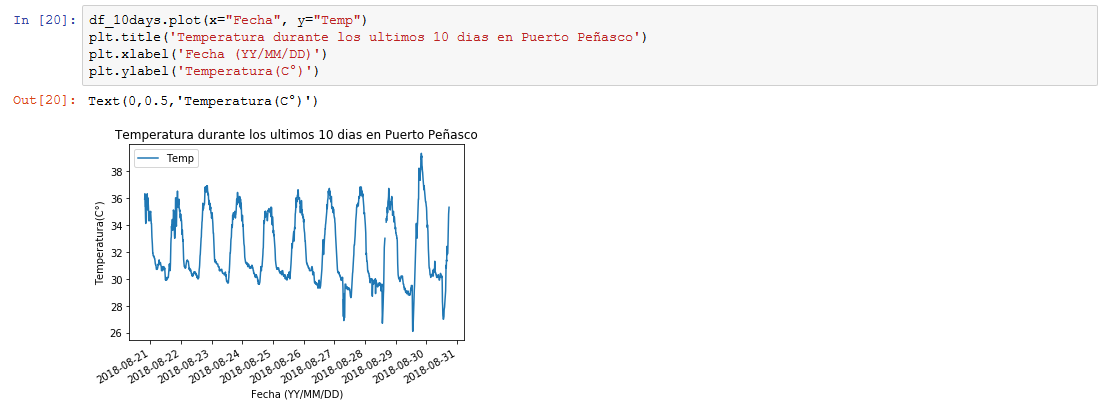
\includegraphics[width=\linewidth]{2-08.png}
\end{figure}
\\
\clearpage
11. Gráfica de la presión en el intervalo de 10 días.
\begin{figure}[h]
  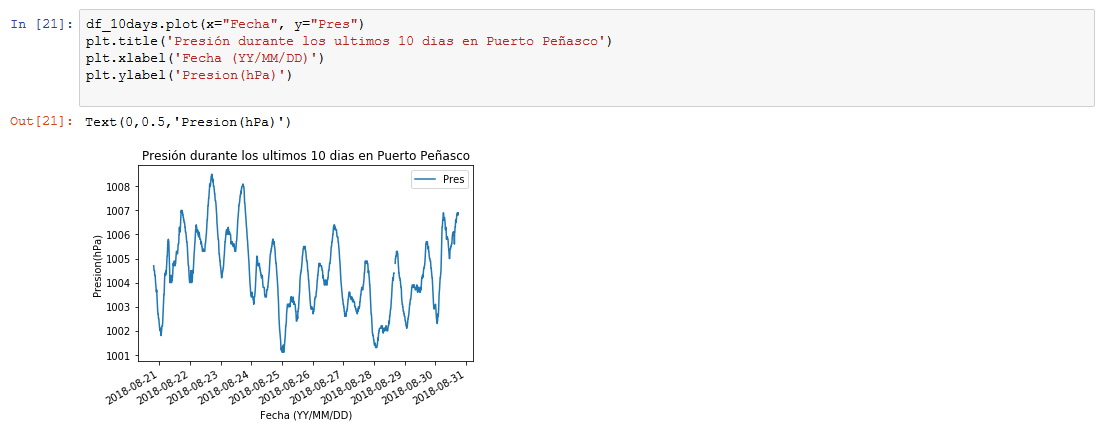
\includegraphics[width=\linewidth]{2-09.png}
\end{figure}

\section{Conclusión}
Realmente al considerar solo 10 días seguidos, no podemos analizar casi cosas, no se mostró casi ninguna variación en la temperatura, y en la presión los cambios no son tan significativos como para concluir que hay un patrón. Pero al fin y al cabo el objetivo de esta actividad era darnos una introducción a Python y su librería de Pandas.


\end{document}
